\documentclass[11pt,onecolumn,titlepage,letterpaper]{article}

\usepackage{cvpr}
\usepackage{times}
\usepackage{epsfig}
\usepackage{graphicx}
\usepackage{amsmath}
\usepackage{amssymb}
\usepackage{mathtools}
\usepackage{array}
\usepackage{multirow}
\usepackage{float}
\usepackage{xcolor}

% Box for the confusion matrix
\newcommand\MyBox[2]{
	\fbox{\lower0.75cm
		\vbox to 1.7cm{\vfil
			\hbox to 1.7cm{\hfil\parbox{1.1cm}{#1#2}\hfil}
			\vfil}%
	}%
}


% Include other packages here, before hyperref.

% If you comment hyperref and then uncomment it, you should delete
% egpaper.aux before re-running latex.  (Or just hit 'q' on the first latex
% run, let it finish, and you should be clear).
\usepackage[breaklinks=true,bookmarks=false]{hyperref}

\cvprfinalcopy % *** Uncomment this line for the final submission

\def\cvprPaperID{****} % *** Enter the CVPR Paper ID here
\def\httilde{\mbox{\tt\raisebox{-.5ex}{\symbol{126}}}}


% Pages are numbered in submission mode, and unnumbered in camera-ready
%\ifcvprfinal\pagestyle{empty}\fi
\setcounter{page}{1}
\begin{document}

%%%%%%%%% TITLE
\title{Using Instagram and ImageNet pretrained deep convolutional networks for seedling species image classification}

\author{Julian Cabezas Pena\\
Student ID: a1785086\\
University of Adelaide, SA 5005 Australia\\
Prepared for COMP SCI 7209 Big Data Analysis and Project \\
{\tt\small julian.cabezaspena@student.adelaide.edu.au}
% For a paper whose authors are all at the same institution,
% omit the following lines up until the closing ``}''.
% Additional authors and addresses can be added with ``\and'',
% just like the second author.
% To save space, use either the email address or home page, not both
}

\maketitle
%\thispagestyle{empty}


%%%%%%%%% ABSTRACT
\begin{abstract}
In the latest years, the field of image classification has been dominated by the use of deep convolutional neural
networks, that have pushed the state of the art in several classification tasks and competitions. These kind of
neural networks contains several parameters that require high computational power and data to train. One of
the common solutions for this problem is the use of transfer learning, that consists in pretraining the model
parameters using a large and known dataset, to then fine tune the model for a specific task. The most commonly
used dataset for pretraining is the ImageNet1k, but in the last years, a database of tagged Instagram images, that
contains billions of images, has been also tested, showing good results, this approach is called Weakly Supervised
Learning, as the Instagram images are tagged by the users of the social network and can contain errors. In
this research, the use of ResNet and ResNeXt neural network architectures, pretrained using the ImageNet or
Imagenet+Instagram datasets were tested to generate a model to predict the prant seedling species from images,
covering 12 distinct weed and crop species, as part of the ”Seedling plant classification” challenge in the Kaggle
website. Four combinations of models and pretraining were tested: i) ResNet-101 with ImageNet pretraining ii)
ResNeXt-101 32x8d with ImageNet pretraining iii) ResNeXt-101 32x8d with Instagram and ImageNet pretraining
iv) ResNeXt-101 32x16d with Instagram and ImageNet pretraining. The learning rate hyperparameter was tuned
in all cases, training the last fully connected layer in 20 epochs and the full neural network in the next 20 epochs.
Additionally, the best performing model was further adjusted in term of data augmentation and batch size. The
results indicate that all the tested models produce very good results in the validation data (above 96\% accuracy),
with the ResNeXt-101 32x16d with Instagram and ImageNet pretraining model being picked for fine-tuning as it
showed more balanced accuracies in the prediction of specific species (Black-grass). With further learning rate
tuning and doubling the amount of epochs, the model reached 97.90\% on the validation data. The results in the
test data (Kaggle submission) showed that the best performing model was the ResNeXt-101 32x8d with ImageNet
pretraining, showing a weighted F1-score of 0.97858 (97.858\% overall accuracy) performance, that would have
corresponded to a position 149 in the leaderboard, reaching the top 20\% performance. This research showed that
pretraining can be a viable and powerful alternative for seedling image classification, with the Instagram dataset
pretraining not producing better results than the ”traditional” Imagenet pretraining.
\end{abstract}


%%%%%%%%% BODY TEXT
\section{Introduction}

In the field of machine learning  and pattern recognition, classification problems are one of the most common approached tasks. In these kind of problems, an algorithm takes a vector of data, and assigns it to one or many discrete classes \cite{Bishop2006}. One of the fields where classification algorithms are extensively used is the field of image classification, where fast improvements in the field have been driven by an accelerated development of the web, that each day generates an immense amount of image data. The field of image classification aims to organize imagine data into a limited amount of classes, based on the characteristics or features of the image. \cite{Zhang2019}

In the last decade, the field of image classification has been dominated by the use of deep convolution networks, that could in some occasions halve the error rate of previously used methods \cite{Krizhevsky2017}, such as the Perceptron \cite{Rosenblatt1957} or Support Vector Machine (SVN) \cite{Vapnik1995}. A convolution neural network is typically defined as a neural network that presents one or more convolutional layers. A convolutional layer is a neuron than covers an adjacent portion of an image, typically groups of 3x3 or 5x5 pixels, transforming the image using a shared set of weights . This technique can cause a major reduction of the number of parameters when comparing it with fully connected neural networks \cite{Aghdam2017}.

The first convolutional neural network to archive the state of the art in image classification was the AlexNet, that uses five convolution layers of different sizes, followed by max pulling layers. This neural network finishes with three fully connected layers, that output the predicted class \cite{Krizhevsky2012}. Short afterwards, this neural network was followed by the Visual Geometry Group (VGG) family of neural networks, that introduced the use of a bigger number a series of very small (3x3 pixels) convolutional layers (19 layers in the deeper version), archiving the state of the art in the ImageNet Large-Scale Visual Recognition Challenge (ILSVRC) of 2015 \cite{Simonyan2015}

A big improvement in terms of neural network deepness was produced with the appearance of the residual networks (ResNet), that managed to solve the gradient vanishing problem. The gradient vanishing is a recurrent issue in deep neural networks, that refers to the problem that occurs when, thought the process of gradient descent, the weight updates became smaller as the layer is farther from the output layer, due to the repeated derivation of the functions that are involved in the process of backpropagation \cite{Aghdam2017,Skansi2018}. To approach this phenomena, the ResNet presents the concept of residual learning, that implies a shortcut or skipping between blocks of layers (residual blocks) \cite{He2016,He2016a}.

Residual networks, as well as other very deep neural networks, can produce very accurate results, but usually require a long time and extensive resources to train. Moreover, these models require big amounts of data to train, thus, a general a common formula is used: First, the convolutional network is trained in a known large annotated image dataset, and secondly, the neural network is fine-tuned using a smaller dataset specific for the classification task to perform \cite{Mahajan2018}. This can be seen as a efficient weight initialization technique, as the model is started with previously learned weights . The use of this approach is often denominated as transfer learning, as the weights of a pretrained model are transferred to a untrained network, avoiding the training of the neural network from scratch \cite{Wani2019}, usually greatly reducing training time and improving performance \cite{Kolesnikov2019}. The extended use of this transfer learning has produced that frameworks for deep learning contain commonly used neural network architectures with the parameters already pretrained using large datasets.

The most common database to perform pretraining of deep convolutional neural networks is the ImageNet Large Scale Visual Recognition Challenge set of images \cite{Russakovsky2015}. This complete dataset contains roughly 14M images comprising 21K categories, although for pretraining, a subset of the dataset, containing one thousand categories and approximately 1.2M labelled images is used. This dataset is used in the annual ILSVRC competition. Although the use of this dataset to pretrain models has produced successful results in several areas, such as image classification, object detection and image segmentation \cite{Huh2016}, in the last years, the Facebook research group proposed an alternative to the ImageNet dataset for transfer learning purposes, using a dataset of billions of Instagram tagged images, in an approach that was called Weakly Supervised Pretraining, as the quality of the labels produced by the Instagram users can have present a low quality, that can be balanced by the amount of data produced, that is several orders of magnitude larger than previous approaches \cite{Mahajan2018}. The use of the Instagram dataset to pretrain models was tested in a variation of the ResNet architectures, called ResNeXt, that produced slightly better results than the standard ResNet in several classification tasks \cite{Xie2017}

One of the uses of these pretrained model is the classification of plant species based on images. This field can have various applications, including automatic weed removal \cite{Giselsson2017} or to support the generation of botanical baseline for environmental impact assessment. The objective of this project is to test and compare the use of ImageNet (IN) and the Instagram (Ins) datasets to train deep convolutional neural network for plant seedling classification, using the "Plant Seedlings Classification" competition in the Kaggle website to asses the performance of two different architectures (ResNet and ResNeXt) using two different pretraining methods (Imagenet or Instagram+Imagenet).


%-------------------------------------------------------------------------


\section{Seedling classification dataset and competition}

The goal of this project is to develop a classification model for seedling images. that correctly predict the species of a seedling from 12 commonly crop and weed species. The database that was used for this purpose is called "Plant Seedling Dataset", and was developed in the University of Southern Denmark and the Aarhus University\cite{Giselsson2017}. This dataset  was designed to act as a benchmark for plant species classification algorithms. The database contains annotated RGB images of approximately 10 pixels per mm., comprising 12 species in different stages of their early development (seedlings). The dataset was developed to asses species classification and also to aid in the design of automatic site-specific weed-control \cite{Giselsson2017}. Examples of the images contained in the dataset can be found in Figure \ref{fig:samples}

\begin{figure}[h]
	\begin{center}
		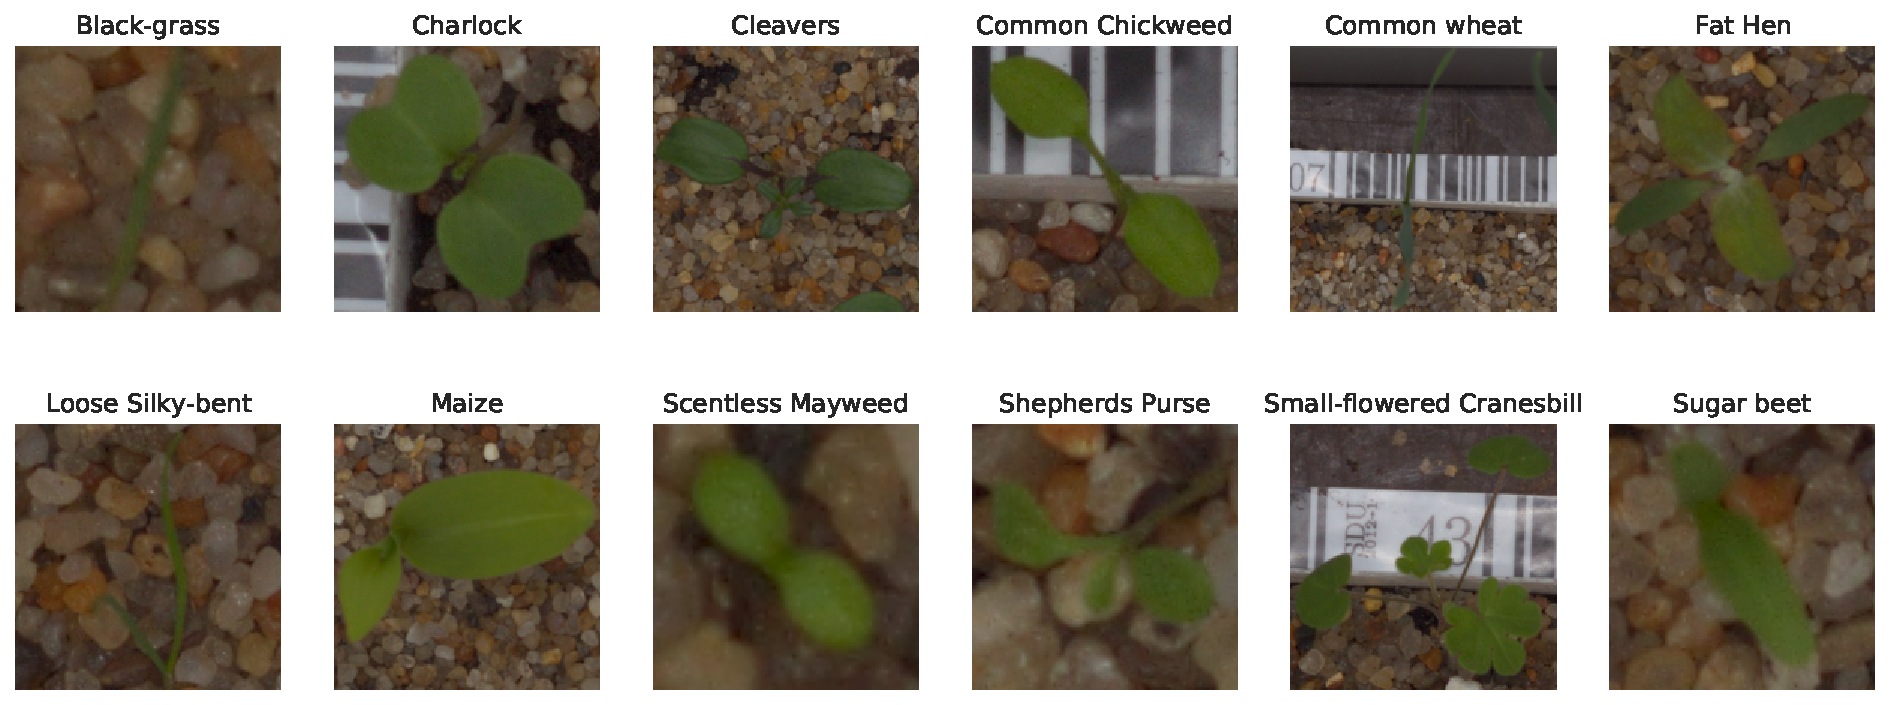
\includegraphics[width=0.9\linewidth]{samples_images.pdf}
	\end{center}
	\caption{Samples of the 12 classes (species) contained in the Plant Seedlings Dataset}
	\label{fig:samples}
\end{figure}

This dataset is the input data for the "Plant Seedlings Classification" competition in the Kaggle website (\url{www.kaggle.com}), were participants are encouraged to apply image classifications techniques to generate the best possible classification. The competition was held in 2017 and measured the model performance using a weighted F1 score metric. The train data contains 4750 labelled images, that are unevenly distributed between the 12 species, as shown in Figure \ref{fig:distribution}. 

\begin{figure}[h]
	\begin{center}
		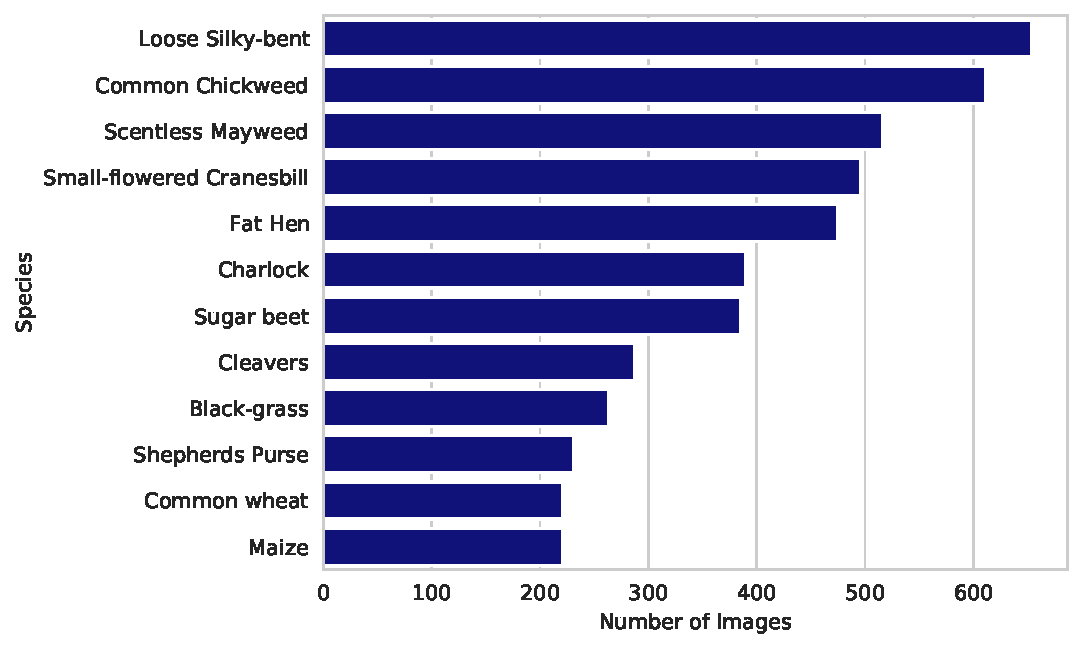
\includegraphics[width=0.8\linewidth]{species_freq.pdf}
	\end{center}
	\caption{Species distribution of the image samples of the Plant Seedlings Dataset}
	\label{fig:distribution}
\end{figure}

On the other side, the test dataset contains 794 unannotated images. The objective of the competition is to predict the species contained in the test data, and to submit it to the Kaggle competition, where the weighted F1 score is computed and a position in the leaderboard was assigned.

\section{Methods}

\subsection{Data Augmentation}

Data augmentation techniques are very important to avoid overfitting and to take advantage of small datasets \cite{Shorten2019}, such as the Plant Seedling dataset. In this case, the following augmentation techniques were used in the train data:

1. \textbf{Random Resized Crop}: In order to modify the scale and set an stable size for the image, the scale was modified using a random value from 0.08 to 1.0, and then cropped to a fixed size of 224x224 pixels, as in Xie \textit{et al} \cite{Xie2017}

2. \textbf{Random Horizontal Flip}: This simple flipping data augmentation technique consists in a 180 degree flipping over the horizontal axis of the image., It has proven effective in several prediction tasks, such as ImageNet and CIFAR-10 \cite{Shorten2019}, in this case, the probability of this data augmentation occurring was set to 0.5 (half of the images)

3. \textbf{Random Clip}: Random cropping or clipping can be a very effective way to simulate the effect of a translation or a feature not being in the centre \cite{Shorten2019}. In this case, a random padding with a maximum of 10 pixels was used, and then the image was clipped to preserve its dimensions (224x224), filling the padded pixels with zero values.

4. \textbf{Image normalization}: Finally, in order to use the ResNeXt and ResNet architectures, a standard normalization  of the images was required, as stated in the documentations of the model \footnote{\url{https://pytorch.org/hub/pytorch_vision_resnext/}} \footnote{\url{https://pytorch.org/hub/pytorch_vision_resnet/}}. Thus, the images were normalized using $mean = {0.485, 0.456, 0.406}$ and $std = {0.229, 0.224, 0.225}$ 

In the case of the validation and test data, the images were resized to 256x256 and then cropped on the centre, to match the size of the input images of the predefined neural networks (224x224), together with the image normalization procedure, following the practices defined in He \textit{at al}  \cite{He2016}.

\subsection{Neural networks architectures and pretraining}

As above mentioned, ResNets solved the vanishing or exploding gradient problem by implementing residual blocks, that add the output of the previous layer to the layer ahead of the block (identity function) (Figure \ref{fig:resnet}). In practice this means this neural networks can be trained using more layers than what previously presented in architectures such as VGG, implementing ResNets of more than one thousand layers and pushing the limits of was considered depth in the CNN area \cite{He2016,He2016a}. These neural networks are often used in transfer learning, producing good results in several image classification tasks \cite{Huh2016}

A variation of the ResNet architecture, called ResNeXt, was recently implemented by the Facebook research group \cite{Xie2017}. This neural network architecture is constructed by repeating a building block, that contain a set of aggregated transformations, forming a multi-branch architecture. In Figure \ref{fig:resnet}, it is possible to appreciate, that the layers in the blocks share the same topology and hyperparameters (filter size and width). As mentioned by Xie \textit{et al} \cite{Xie2017}, the ResNet architectures stack a set of modules of the same topology, creating a "essential" dimension that can in some cases produce a over adaptation of hyperparameters for specific datasets. On the other size, the ResNeXt architectures include a new dimension called "cardinality" (C) (size of the set of transformations), that can be more effective than creating a deeper network, while maintaining the complexity of the model \cite{Xie2017}.


\begin{figure}[h]
	\begin{center}
		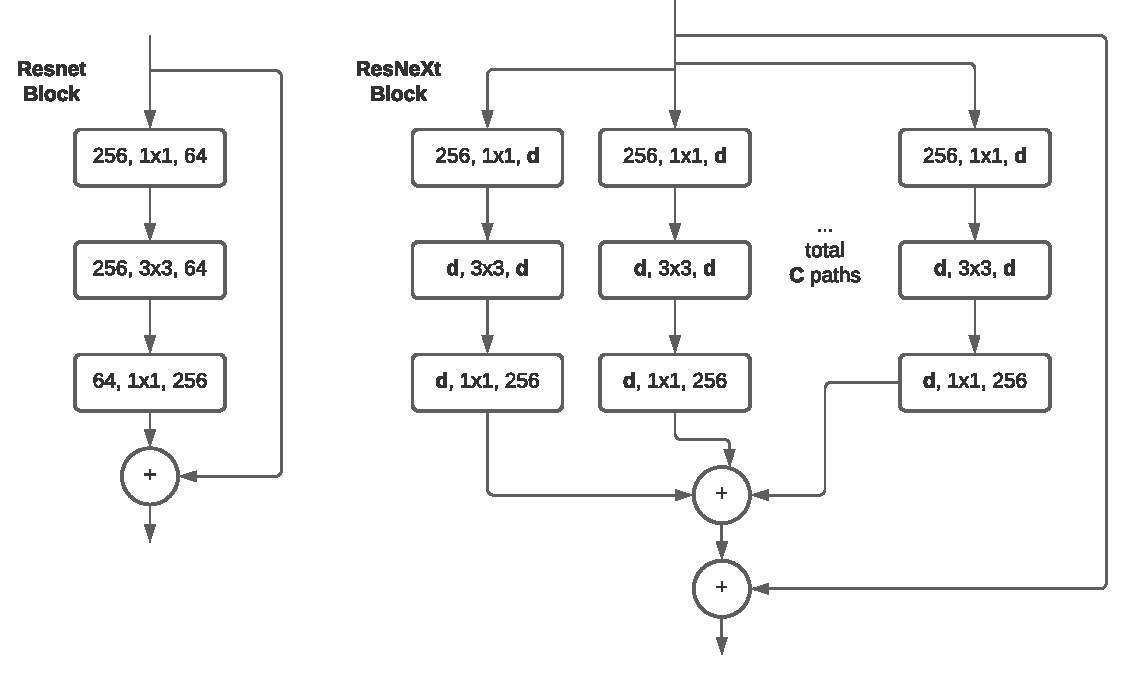
\includegraphics[width=0.8\linewidth]{resnet_resnext_block.pdf}
	\end{center}
	\caption{ResNet and ResNeXt block. C = Cardinality, d = bottleneck, The layer are shown as (number of \textit{in} channel, filter size, number of \textit{out} channels). Adapted from Xie \textit{et al} \cite{Xie2017}}
	\label{fig:resnet}
\end{figure}

In order to test different neural network architectures and pretraining methods, four combinations of the two above mentioned neural networks and pretraining methods were tested:

\textbf{ResNet101 - ImageNet (IN) pretrained}: In order to have a baseline of one of the most common architectures and pretrained method, a ResNet of 101 layers was tested. This architecture was the state of the art for the CIFAR-10 dataset when it appeared, showing a 6.43\% error, and the 152 layer variant of this neural network architecture was the winner of the ILSVRC 2015 challenge, with 19.38\% of top-1 error and 4.49\% of top 5 error \cite{He2016}. This architecture was pretrained on the ImageNet1K dataset.

\textbf{ResNeXt-101-32x8d - ImageNet (IN) pretrained}: A ResNeXt architecture, also containing 101 layers, was implemented. This neural network architecture replaces the blocks present in ResNet-101 with ResNeXt blocks of cardinality = 32 and bottleneck width = 8 (hence the 32x8d nomenclature). According to Xie \textit{et al}, this kind of architecture outperforms the equivalent ResNet-101 in ImageNet1K classification \cite{Xie2017}. This architecture was also pretrained on the ImageNet1K dataset.

\textbf{ResNeXt-101-32x8d - Instagram (Ins) + ImageNet (IN) pretrained}: The same ResNeXt-101 32x8d architecture was tested, but this variant was firstly pretrained using a dataset of roughly one billion Instagram tagged images. According to the Facebook research authors \cite{Mahajan2018}, the inclusion of the Instagram dataset can produce a 1.5\% accuracy boost compared with the ImageNet pretrained network, when using the model in tasks such as CUB2011 or Places365. This neural network was firstly pretrained using the Instagram (Ins) dataset, to then train it with the ImageNet1K dataset.

\textbf{ResNeXt-101-32x16d - Instagram (Ins) + ImageNet (IN) pretrained}: In order to test a more complex ResNeXt architecture, the bottleneck (d) with was increased to 16 (Figure \ref{fig:resnet}), as according to Mahajan \textit{et al} \cite{Mahajan2018}, this architecture accomplishes the best accuracy in the CUB2011m ImageNet 1k, 5k and 9k classification tasks.

In all cases, the only modification that was performed was replacing the last fully connected layer, that outputs 1000 values (as all af them are trained using the ImageNet1K classification in mind) with a fully connected layer with output=12, as the seedling database contains that amount of distinct species.

\subsection{Neural network training}

According to Wani \textit{et al}, \cite{Wani2019}, the use of transfer learning usually follows two methodologies:  \textit{(i) Use the pretrained neural network as a feature extractor}: In this case only the last fully connected layer is replaced with a new classifier and only that layer is trained, keeping the rest of the neural network "frozen" \textit{(ii) Train the whole neural network}: In this case, the last fully connected layer is also replaced but the totality of the model is trained through backpropagation.

In order to take advantage of both approaches, in this study the neural networks were trained using two stages. In the first stage, 20 epochs were used to train the last fully connected layer (classifier), and then the totality of the neural network was trained using backpropagation in the next 20 epochs. 

In order to prevent gradient explosion \cite{Aghdam2017}, different learning rates were used in the two stages of training. Thus, the learning rate used in the first stage (tuned hyperparameter) was then multiplied by a factor of 0.1 in the second stage (e.g. if the learning rate in the first stage was 0.01 in the second stage it was 0.001). Additionally, the initial learning rate was decreased using a 0.1 multiplier factor every 7 steps in order to fine-tune the parameters of the neural network, as in Mahajan \textit{et al} \cite{Mahajan2018}


\subsection{Loss function and optimization criterion}

To get the predicted value of the neural network, a Softmax function, that takes the last output of the last neural network, was used:

\begin{equation}
	{Softmax}(x_{i}) = \frac{\exp(f(x_i))}{\sum_{j=1}^{m} \exp(f(x_j))}
\end{equation}

where $x_i$ is the $i$ output element result of the last fully connected layer of the neural network, and $m$ is the number of classes. As the function includes a division by the sum of the exponentials of the outputs. The sum the Softmax output values is always 1 \cite{Skansi2018}.

To calculate the loss in each batch, the cross-entropy function for a set of parameters $\theta$ is used \cite{Hastie2009}:

\begin{equation}
	{Loss}(\theta) = - \sum_{i=1}^{n} y_i log(f(x_i))
\end{equation}

where $y_i$ is the one-hot encoded vector of true labels and $n$ the number of elements in the mini-batch. 

Using this loss function, backpropagation on a minibatch of size 10 was used to update the parameters of the neural network, for the this purpose, the Adam optimizer was applied. The Adam optimizer was introduced by Kingma and Ba \cite{Kingma2015} and provides a computationally efficient method for stochastic optimization, suitable for noise and sparse gradients.

\subsection{Hyperparameter tuning}

One of the most important steps in the implementation of deep learning models is the tuning or adjusting of hyperparameters \cite{Skansi2018}. To avoid overfitting, the train data was randomly splitted into a training (75\%) and a validation set (25\%). Then, different hyperparameter were tested by training the neural in the train set and measuring the overall accuracy in the validation set. In this case, as four models were tested and the computation hardware was limited, initially only the learning rate was tuned for all models, testing three possible starting learning rates (0.001, 0.003 and 0.005). 

In the case of the model with a better performance, a fine-tuning of the learning rate was performed by analysing the loss curves, to then tune the batch size, using batch sizes equal to 10, 20 and 30 images and to test additional data augmentation methods. Finally, the a greater number of epochs (80) was tested in the case of the model showing the best performance on the validation set, to build a fine tuned model.

\subsection{Model testing}

In order to asses the model performance in a real world situation, the complete train dataset was used to train the the final models, using the best performing learning rate. This trained model as then used to predict the species of the seedling images contained in the test set. The predicted labels were submitted to the Kaggle website of the competition (\url{https://www.kaggle.com/c/plant-seedlings-classification/}), were a weighted F1 score was calculated, that in this case is equal to the Overall Accuracy. As the competition was finished on 2017, the position on the leaderboard was calculated by looking at the public leaderboard produced at the end of the competition, allowing to asses the accuracy of the model with respect to other Kaggle competitors.

\section{Results and Discussion}

\subsection{Learning rate tuning}

As shown in Figure \ref{fig:lr}, the three combinations of learning rate tend to give similar results in the first stage of training, although in epoch 20 (change between the training of the last fully connected layer and the training of the full neural network), a drop in accuracy is present, this drop can be caused by a gradient explosion \cite{Aghdam2017}, and it has a greater magnitude in the ResNeXt architectures pretrained with the Instagram datasets, where, with a learning rate of 0.0005. the training and validation accuracies drop from approximately 80\% to less than 40\% in both cases.

\begin{figure}[h]
	\begin{center}
		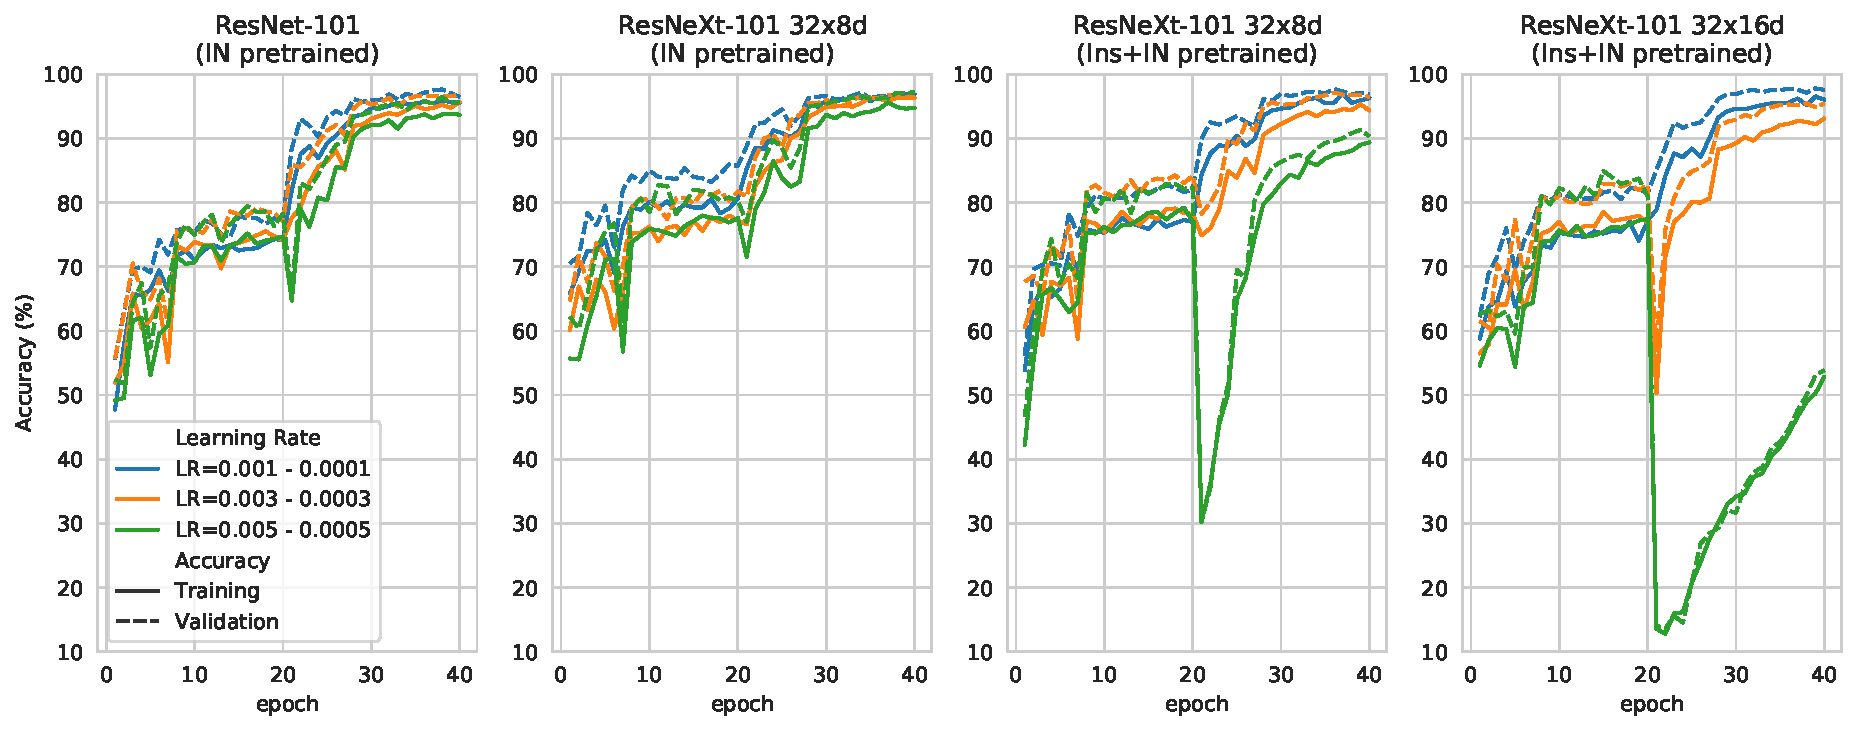
\includegraphics[width=1.0\linewidth]{lr_4models.pdf}
	\end{center}
	\caption{Training and Validation accuracy of the four models using different learning rates. Ins = Instagram, IN = ImageNet1K}
	\label{fig:lr}
\end{figure}

This accuracy drop is better represented in the loss curves (Figure \ref{fig:loss}), where the cross entropy loss clearly reflects a severe spike when the 0.003-0.0003 and 0.005-0.0005 learning rates are used. These results show that the optimal learning rate for all the tested neural network architectures is 0.001 in the first stage and 0.0001 in the next step.

\begin{figure}[h]
	\begin{center}
		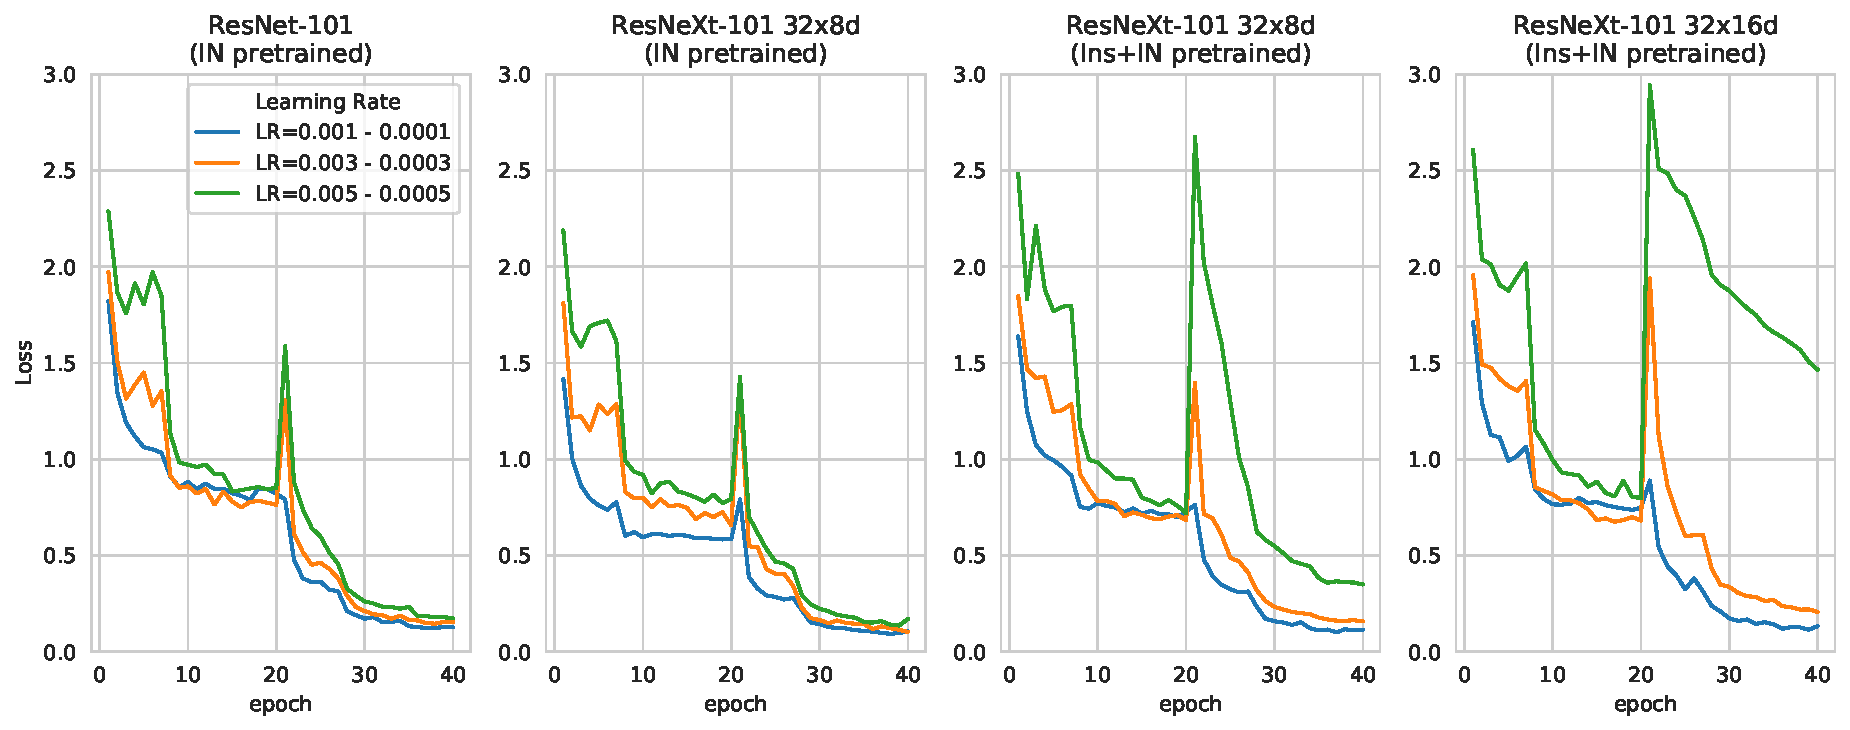
\includegraphics[width=1.0\linewidth]{loss_4models.pdf}
	\end{center}
	\caption{Loss curves of the four models using different learning rates. Ins = Instagram, IN = ImageNet1K}
	\label{fig:loss}
\end{figure}

\subsection{Validation set performance}

The performance of the four models models was measured in the validation data, and represented as per-class accuracy in Table \ref{table:val}. In that Table, it is possible to see that all models reach a similar overall accuracy, ranging from 96.80\% in the case of the ResNet-101 (IN pretrained) to 96.63\% in the ResNeXt-101 32x8d (Ins+IN Pretrained) model.

As this database presents an uneven number of species per class (Figure \ref{fig:distribution}), the overall accuracy can be overly influenced by the classes that contain more samples such as the Loose Silky-bent and the Common Chickweed, where accuracies of the Maize and Common wheat species can be under-represented in the overall accuracy metric. On the other side, by looking at the specific class accuracies (Table \ref{table:val}), it is possible to see that all models present their worst accuracy in the Black-grass species. In this case, the best performing model is the ResNeXt-101 32x16d (Ins+IN Pretrained) neural network, that reaches 85\% accuracy in this class. Given this result, this model was picked for fine-tuning, because it is important to have balanced class accuracies to develop a useful model.

\begin{table}[h]
	\begin{center}
		\begin{tabular}{|p{4.1cm}|p{2.8cm}|p{2.8cm}|p{2.8cm}|p{2.8cm}|}
			\hline
			Class & ResNet-101 (IN Pretrained) & ResNeXt-101 32x8d (IN Pretrained) & ResNeXt-101 32x8d (Ins+IN Pretrained) & ResNeXt-101 32x16d (Ins+IN Pretrained)\\
			\hline\hline
			Black-grass &  \textcolor{red}{76.67\%} &\textcolor{red}{81.67\%}  & \textcolor{red}{76.67\%}  & \textcolor{red}{85.00\%}  \\
			Charlock & 100.00\% & 100.00\% & 100.00\% & 100.00\% \\
			Cleavers & 95.89\% & 97.26\% & 98.63\% & 100.00\%  \\
			Common Chickweed & 100.00\% & 98.51\% & 100.00\% & 99.25\%\\
			Common wheat & 96.43\%  & 98.21\% & 96.43\% & 92.86\%\\
			Fat Hen & 100.00\% & 99.21\% & 99.21\% & 99.21\% \\
			Loose Silky-bent & 95.83\% & 97.62\% & 92.26\% & 92.86\% \\
			Maize & 98.18\% & 100.00\% & 100.00\% & 100.00\% \\
			Scentless Mayweed & 97.71\% & 97.71\% & 97.71\% & 97.71\% \\
			Shepherds Purse & 89.83\% & 96.61\% & 94.92\% & 100.00\% \\
			Small-flowered Cranesbill & 100.00\% & 100.00\% & 98.46\% & 99.23\% \\
			Sugar beet & 98.02\% & 96.04\% & 99.01\% & 97.03\% \\
			\hline
			\textbf{Overall accuracy} & \textbf{96.80\%} & \textbf{97.47\%} & \textbf{96.63\%} & \textbf{97.14\%} \\
			\hline
		\end{tabular}
	\end{center}
	\caption{Models accuracy in the validation data, the worst class accuracy is represented in red}
	\label{table:val}
\end{table}

When analysing the confusion matrix of the ResNeXt-101 32x16d (Ins+IN Pretrained) for the validation data (Figure \ref{fig:cm}), it is possible to appreciate a big proportion of the samples are well classified. Although the the model confuses the Black-grass with the Loose Silky-bent, affecting the accuracies of both classes. Thought the confusion between the two species is not surprising, as both species belong to the \textit{Poaceae} family of species, that corresponds to a particularly hard to identify taxonomic group (even for experienced botanists) \cite{Nesbitt2016}. Furthermode, this model could be employed to design an automatic weed remover, as suggested by Giselsson \textit{et al} \cite{Giselsson2017}, as both species are considered as weeds for agricultural production purposes.

\begin{figure}[h]
	\begin{center}
		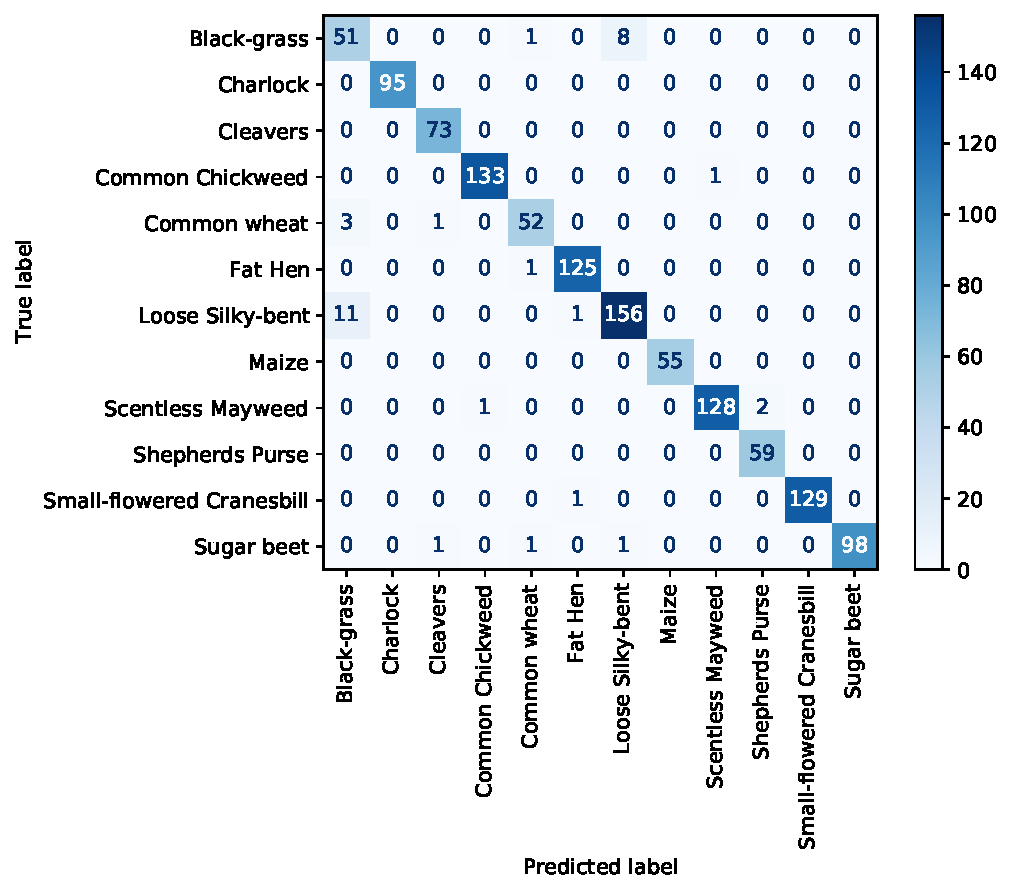
\includegraphics[width=0.65\linewidth]{confusion_matrix.pdf}
	\end{center}
	\caption{Confusion matrix for the ResneXt-101 32x16d model (Instagram + Imagenet1K Pretrained) predictions on the validation data}
	\label{fig:cm}
\end{figure}

\subsection{Further hyperparameter tuning}

As the ResNeXt-101 32x16d (Ins+IN Pretrained) showed the most balanced results overall, additional hyperparameter combinations and data augmentations methods were tested (Table \ref{table:finetune}). In this case, as the photographs of the dataset were taken from above, a random vertical flip was tested, but it did not improved the results. Additionally, random a modification of the hue, saturation, brightness and contrast were tested (ColorJitter data augmentation method) \cite{Shorten2019}, also without producing better results.

A slightly smaller learning rate (0.000075) in the second stage of the training (training of the whole neural network) was tested, as the loss increases in the transition between both stages (Figure \ref{fig:loss}. This new learning rate slightly increased the overall accuracy (from 97.14\% to 97.73\%). With this new learning rate, bigger batch sizes (15 and 20) were tested, without improvements. Finally, the neural network was tested using 80 epochs (40 in each stage), also showing a small improvement in the validation accuracy (97.90\%) (Table \ref{table:finetune}.

\begin{table}[h]
	\begin{center}
		\begin{tabular}{|p{2.8cm}|p{2.8cm}|p{2.8cm}|p{2.8cm}|p{2.8cm}|}
			\hline
			Additional data augmentation & Batch size & Learning rates & Number of epochs & Validation set overall accuracy \\
			\hline\hline
			Vertical Flip & 10 & 0.001 - 0.0001 & 40 & 96.80\% \\
			Color Jitter & 10 & 0.001 - 0.0001 & 40 & 96.46\%  \\
			- & 10 & 0.001 - 0.000075 & 40 & 97.73\% \\
			- & 15 & 0.001 - 0.000075 & 40 & 97.14\%  \\
			- & 20 & 0.001 - 0.000075 & 40 & 97.14\%  \\
			\textbf{-} & \textbf{10} &\textbf{0.001 - 0.000075} & \textbf{80} & \textbf{97.90\%}  \\
			\hline
		\end{tabular}
	\end{center}
	\caption{Performance of the models in the test data (Kaggle submission)}
	\label{table:finetune}
\end{table}

The confusion matrix of this model (Figure \ref{fig:cm2}) shows that this neural network produces slightly less misclassification between Black-grass with the Loose Silky-bent, improving previous results. Although this results could be considered as an improvement, the accuracy gain resulting from further adjusting of hyperparameters and data transformation did not produce a improvement worth the effort and training time, increasing less than 0.5\& overall accuracy compared with other not so fine tuned models such as ResNeXt-101 32x8d (Ins+IN Pretrained), showing that in this case, the tuning of the learning rate was one of the most important hyperparameters \cite{Hastie2009}, together with the inclusion of standard data augmentation methods \cite{Shorten2019}.

\begin{figure}[h]
	\begin{center}
		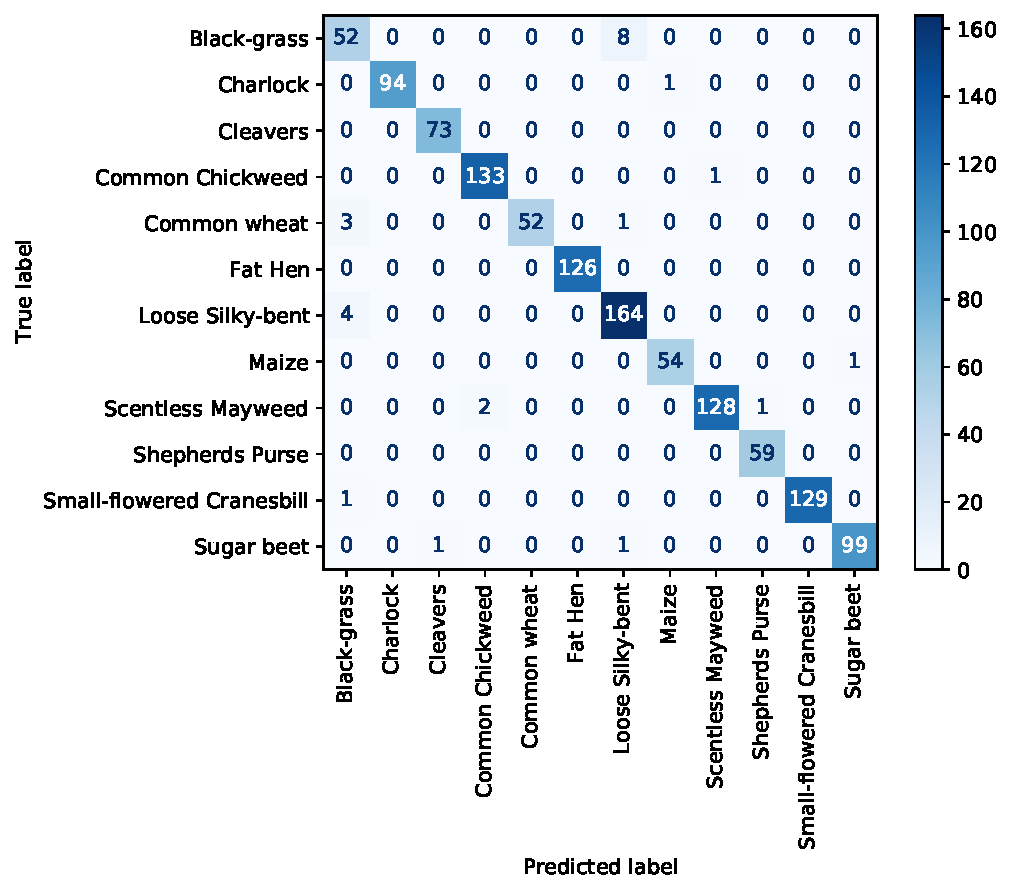
\includegraphics[width=0.65\linewidth]{confusion_matrix_finetune.pdf}
	\end{center}
	\caption{Confusion matrix for the fine tuned ResneXt-101 32x16d model (Instagram + Imagenet1K Pretrained) predictions on the validation data, using 40 epochs and LR = 0.001 - 0.000075}
	\label{fig:cm2}
\end{figure}

\subsection{Testing results}

When getting the prediction on the test set and submitting them to Kaggle, it is possible to see that the best performing model is the ResNeXt-101 32x8d model that was pretrained only using the ImageNet1K dataset, that presents a weighted F1 score of 0.97858 (97.86\% overall accuracy) (Table \ref{table:test}), with that performance, this model would have reached position 149 in the leaderboard, being on the top 20\% best performing models of the competition. This model is closely followed by the same architecture (ResNeXt-101 32x8d) pretrained using the Instagram and ImageNet dataset, being very close in terms of performance (0.97732 F1-score) and in the leaderboard (position 173). As the only difference in these two neural network implementation is their pretraining, these results are not consistent to what is mentioned in Mahajan \textit{et al} \cite{Mahajan2018}, that affirms that the weakly supervised learning pretraining made with the Instagram images can produce performance increases in various tasks.

Even though the ResNeXt-101 32x16d showed the best performance in the validation data, in the test data it showed one of the worst performances. Moreover, the fine tuning of parameters, that including double the amount of epochs and a slightly reduced learning rate, produced slightly worst results than the version with only the original learning rate. This results are not coherent with the Xie \textit{et al}  \cite{Xie2017} and Mahajan \textit{et al} \cite{Mahajan2018}, that state that increasing the bottleneck parameter can increase the performance of the ResNeXt models. These results show that probably a slight overfitting effect can be occurring, that is not being reflecting in the validation data, that can present a different species distribution than the test data (that has a unknown species distribution) 

\begin{table}[h]
	\begin{center}
		\begin{tabular}{|p{9.1cm}|p{2.8cm}|p{2.8cm}|}
			\hline
			Model & Mean F1 Score (Overall accuracy) & Simulated Leaderboard position\\
			\hline\hline
			Resnet-101 (IN Pretrained) & 0.97103 & 262/833 (31.45\%) \\
			ResneXt-101 32x8d (IN Pretrained) & 0.97858 & 149/833 (17.89\%)  \\
			ResneXt-101 32x8d (Ins+IN Pretrained) & 0.97732 & 173/833 (20.77\%)   \\
			ResneXt-101 32x16d (Ins+IN Pretrained) & 0.97229 & 248/833 (29.77\%) \\
			ResneXt-101 32x16d (Ins+IN Pretrained) - Fine tuned & 0.96977 & 324/833 (38.90\%) \\
			\hline
		\end{tabular}
	\end{center}
	\caption{Performance of the models in the test data (Kaggle submission)}
	\label{table:test}
\end{table}

On the other hand, these results confirm the findings of Xie \textit{et al} \cite{Xie2017}, that point out that the ResNeXt architectures perform better that equivalent ResNet architectures. In this particular research, this is true in nearly all the cases, where the ResNet-101 is outperformed in the test and validation data.

\section{Conclusion}

This project showed that pretrained deep convolutional neural networks can be a suitable alternative for seedling species classification, reaching competitive performances with minimal hyperparameter adjusting and only using common data augmentation methods. The models produced in this research could be adapted for automatic weed-removal mechanisms, as they only suffer from relevant misclassification between two weed species.

This research also showed that pretraining deep neural networks using the very large and weakly supervised Instagram dataset did not produced better results than using the standard ImageNet1K dataset, contrary with what was mentioned on the literature. On the other side, this research showed the capabilities of the ResNeXt models, that slightly outperformed the traditional ResNet architectures.

Even though different hyperparameters such as batch size, number of epochs and different data augmentation methods were tested without improving the performance of the models, future research could further enhance the prediction capabilities of this model by using other hyperparameter combinations, testing different optimization methods (such as the commonly used Stochastic Gradient Descent with momentum) or generating separate models for the species that are misclassified.


{\small
\bibliographystyle{ieeetr}
\bibliography{library}
}

\end{document}
